\documentclass[12pt,a4paper]{article}
\usepackage{times}
\usepackage{epsf}
\usepackage{bm}
\usepackage{latexsym}
\usepackage{subcaption}
\usepackage[]{graphics}
\usepackage{graphicx}
\usepackage{subcaption}
\usepackage{xcolor}

\title{CS436, HW2, 3 questions, 100 points}
\author{ Gustavo Hammerschmidt\thanks{hamme032@cougars.csusm.edu} \\ California State University San Marcos\\ }


\usepackage{biblatex}
\addbibresource{references.bib}

\begin{document}

\maketitle


Note: b denotes bits and B denotes Bytes (1 Byte = 8 bits).


\textcolor{red}{Question 1: 32 points: (16)+(16)}

\begin{figure}[h!]
  \centering
  \begin{subfigure}[b]{0.8\linewidth}
    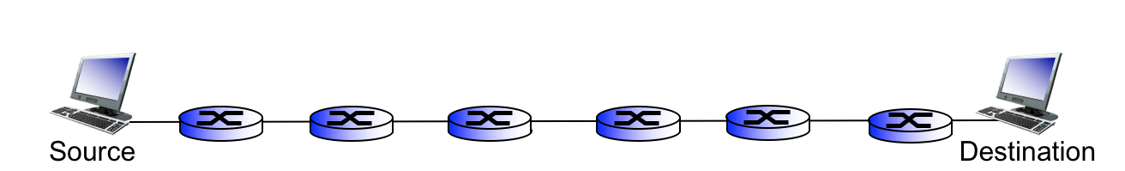
\includegraphics[width=\linewidth]{q1.png}
  \end{subfigure}
  \caption{Question 1 Network}
  \label{fig:coffee}
\end{figure}

Consider a packet of length $L$, which begins at source and travels over seven links to a destination. These links are connected through six routers. Let $d_{i}$, $s_{i}$, and $R_{i}$ denote the length, propagation speed, and the transmission rate of link $i$, for i = 1 to 7. The processing delay at each router is $d_{proc}$. The queuing delay at each router is $d_{que}$. What is the total end-to-end delay for the packet in terms of $d_{i}$, $s_{i}$ , $R_{i}$ ($i$ = 1 to 7), and $L$? 

$
\\
Packet\ Length = L(Length\ must\ be\ in\ bits) 
\\
\\
Length\  link = d_{i} 
\\
Propagation\ speed = s_{i}
\\
Transmission\ rate = R_{i}
\\
\\
Processing\ delay = d_{proc}
\\
Queuing\ delay = d_{que}
\\
\\
Transmission\ delay = \frac{Packet \ Length(bits)}{Transmission \ Rate(bits/sec)} = \frac{L}{R_{i}}
\\
\\
Propagation\ delay = \frac{link's \ length}{propagation \ speed} = \frac{d_{i}}{s_{i}}
\\
\\
$

$\\ \\$

Delay at first link is equal to transmission delay plus propagation delay.

\begin{equation}
First Link = delay_{transmission} + delay_{propagation}
\end{equation}

$\\ \\$

From the second to the last link(seventh), the processing and queuing delay are also considered in the total delay of the link.


\begin{equation}
\sum\limits_{i = 2}^7 \ \ delay_{trans}{\ i} \ + \ delay_{prop}{\ i} \ +
\ delay_{proc}{\ i} \ + \ delay_{que}{\ i} = Total \ delay_{\ \ links\ 2\ to\ 7}    
\end{equation}

$\\ \\$

Conclusion(Final\ Answer):

The end-to-end delay is:


\begin{equation}
\textcolor{red}{end\ to\ end\ delay \ =\ d_{trans}\ +\ d_{prop} + 6 \times (d_{trans} + d_{prop} + d_{proc} + d_{que})}
\end{equation}


Now in Terms of $d_{i}$, $s_{i}$, $R_{i}$ ($i$ = 1 to 7), and $L$:


\begin{equation}
\textcolor{red}{end\ to\ end\ delay \ =\ \sum\limits_{i = 1}^7 \frac{L}{R_{i}} + \frac{d_{i}}{s_{i}} + \sum\limits_{i = 2}^7 d_{proc}{i} + d_{que}{i}}
\end{equation}


The end to end delay is the sum of the transmission and propagation delay sum(from link 1 to link 7) and the processing and queuing delay sum(from link 2 to link 7).

$
\\
\\
$


Now suppose, the packet is \textcolor{purple}{2,500} Bytes, the propagation speed on all links is \textcolor{purple}{$2.5 \times 10^8$} m/s (meters per second), the transmission rates of all links are \textcolor{purple}{1.6} Mbps. The length of first and second links are \textcolor{purple}{5,000} Km (kilometer), the length of third, fourth, fifth and sixth links are \textcolor{purple}{4,000} Km, and the length of seventh links is \textcolor{purple}{1,000} Km. Processing delay in each router is \textcolor{purple}{2} msec (mili-second) and queuing delay in each router is \textcolor{purple}{7} msec. For these values, what is the end-to-end delay? Write down your calculations. 

$
\\
Packet\ Length = 2500\ bytes = 2500 * 8\ bits\\
\\
Length\ of\ links\ 1\ and\ 2\ =\ 5000\ km\\
Length\ of\ links\ 3,\ 4,\ 5\ and\ 6\ = 4000\ km\\
Length\ of\ link\ 7\ =\ 1000\ km\\
Propagation\ speed = 2.5 \times 10^8\ m/s\ (for\ all\ links)\\
Transmission\ rate = 1.6\ Mbps\ (for\ all\ links)\\
\\
Processing\ delay = 2\ msec\\
Queuing\ delay = 7\ msec\\
\\
$

$\\ \\$

Formula for this problem:

\begin{equation}
end\ to\ end\ delay \ =\ \sum\limits_{i = 1}^7 \frac{L}{R_{i}} + \frac{d_{i}}{s_{i}} + \sum\limits_{i = 2}^7 d_{proc}{i} + d_{que}{i}
\end{equation}

$\\ \\$

Processing and queuing delays are the same in each router. The are six routers in the path, therefore, these delays are summed six times:

\begin{equation}
Processing\ and\ queuing\ delay\ (links\ 2\ to\ 7)\ =\ 6\ \times\ (d_{proc}\ +\ d_{que})\\
\end{equation}
\begin{equation}
Processing\ and\ queuing\ delay\ (links\ 2\ to\ 7)\ =\ 6\ \times\ (2\ msec\ +\ 7\ msec)    
\end{equation}
 \begin{equation}
Processing\ and\ queuing\ delay\ (links\ 2\ to\ 7)\ =\ 6\ \times\ (9\ msec)    
\end{equation}
 \begin{equation}
 \textcolor{red}{
Processing\ and\ queuing\ delay\ (links\ 2\ to\ 7)\ =\ 54\ milliseconds}
\end{equation}
 
 
 $\\ \\$
 
The total transmission delay:


\begin{equation}
    Total\ Transmission\ delay\ =\ \sum\limits_{i = 1}^7 link(i) = \frac{Packet\ Length(bits)}{Transmission\ Rate(bits/sec)}
\end{equation}
\begin{equation}
    Total\ Transmission\ delay\ =\ \sum\limits_{i = 1}^7 link(i) = \frac{2500 * 8 bits}{1.6 Mbps}
\end{equation}
\begin{equation}
    Total\ Transmission\ delay\ =\ \sum\limits_{i = 1}^7 link(i) = \frac{2 \times 10^4 bits}{1.6 \times 10^6 b/s}
\end{equation}
\begin{equation}
    Total\ Transmission\ delay\ =\ \sum\limits_{i = 1}^7 link(i) = \frac{2}{1.6}*10^{4-6}\ seconds
\end{equation}
\begin{equation}
    Total\ Transmission\ delay\ =\ \sum\limits_{i = 1}^7 link(i) = 1.25 *10^{-2}\ seconds
\end{equation}
\begin{equation}
    Total\ Transmission\ delay\ =\ \sum\limits_{i = 1}^7 link(i) = 0.125 *10^{-3}\ seconds
\end{equation}
\begin{equation}
    Total\ Transmission\ delay\ =\ 7 \times ( 0.125\ milliseconds)
\end{equation}
\begin{equation}
\textcolor{red}{
    Total\ Transmission\ delay\ =\ 0.875\ milliseconds}
\end{equation}

$\\ \\$

Propagation delay for links 1 and 2 is:
\begin{equation}
    Propagation\ delay\ =\ \frac{Link's\ length}{Propagation speed}
\end{equation}
\begin{equation}
    Propagation\ delay\ =\ \frac{5000\ km}{2,5 \times 10^8\ m/s}
\end{equation}
\begin{equation}
    Propagation\ delay\ =\ \frac{5 \times 10^3\times 10^3\ m}{2,5 \times 10^8\ m/s}
\end{equation}
\begin{equation}
    Propagation\ delay\ =\ \frac{5 \times 10^6\ m}{2,5 \times 10^8\ m/s}
\end{equation}
\begin{equation}
    Propagation\ delay\ =\ \frac{5}{2,5} \times 10^{6-8}\ seconds
\end{equation}
\begin{equation}
    Propagation\ delay\ =\ 2 \times 10^{-2} seconds
\end{equation}
\begin{equation}
    Propagation\ delay\ =\ 0.2 \times 10^{-3} seconds
\end{equation}
\begin{equation}
\textcolor{red}{   Propagation\ delay\ =\ 0.2\ milliseconds}
\end{equation}

$\\ \\$

Propagation delay for links 3, 4, 5 and 6:

\begin{equation}
    Propagation\ delay\ =\ \frac{Link's\ length}{Propagation speed}
\end{equation}
\begin{equation}
    Propagation\ delay\ =\ \frac{4000\ km}{2,5 \times 10^8\ m/s}
\end{equation}
\begin{equation}
    Propagation\ delay\ =\ \frac{4 \times 10^3\times 10^3\ m}{2,5 \times 10^8\ m/s}
\end{equation}
\begin{equation}
    Propagation\ delay\ =\ \frac{4 \times 10^6\ m}{2,5 \times 10^8\ m/s}
\end{equation}
\begin{equation}
    Propagation\ delay\ =\ \frac{4}{2,5} \times 10^{6-8}\ seconds
\end{equation}
\begin{equation}
    Propagation\ delay\ =\ 1,6 \times 10^{-2} seconds
\end{equation}
\begin{equation}
    Propagation\ delay\ =\ 0.16 \times 10^{-3} seconds
\end{equation}
\begin{equation}
\textcolor{red}{    Propagation\ delay\ =\ 0.16\ milliseconds}
\end{equation}

$\\ \\$

Propagation delay for link 7:


\begin{equation}
    Propagation\ delay\ =\ \frac{Link's\ length}{Propagation speed}
\end{equation}
\begin{equation}
    Propagation\ delay\ =\ \frac{1000\ km}{2,5 \times 10^8\ m/s}
\end{equation}
\begin{equation}
    Propagation\ delay\ =\ \frac{1 \times 10^3\times 10^3\ m}{2,5 \times 10^8\ m/s}
\end{equation}
\begin{equation}
    Propagation\ delay\ =\ \frac{1 \times 10^6\ m}{2,5 \times 10^8\ m/s}
\end{equation}
\begin{equation}
    Propagation\ delay\ =\ \frac{1}{2,5} \times 10^{6-8}\ seconds
\end{equation}
\begin{equation}
    Propagation\ delay\ =\ 0,4 \times 10^{-2} seconds
\end{equation}
\begin{equation}
    Propagation\ delay\ =\ 0,04 \times 10^{-3} seconds
\end{equation}
\begin{equation}
\textcolor{red}{    Propagation\ delay\ =\ 0.04\ milliseconds}
\end{equation}

$\\ \\$

Total Propagation Delay(sum of links 1 to 7):

\begin{equation}
    Total\ Propagation\ delay\ =\ d_{prop}{\ links\ 1\ and\ 2\ }\ +\ d_{prop}{\ links\ 3,\ 4,\ 5\ and\ 6\ }\ +\ d_{prop}{\ link\ 7}
\end{equation}
\begin{equation}
    Total\ Propagation\ delay\ =\ 2 * (0.2\ ms)\ +\ 4 * (0.16\ ms)\ +\ 1 * (0.04\ ms)
\end{equation}
\begin{equation}
    Total\ Propagation\ delay\ =\ (0.4\ ms)\ +\ (0.64\ ms)\ +\ (0.04\ ms)
\end{equation}
\begin{equation}
    \textcolor{red}{ Total\ Propagation\ delay\ =\ 1.08\ milliseconds}
\end{equation}

$\\ \\$

The end-to-end delay is the sum of all the propagation, processing, queuing and transmission delays:

\begin{equation}
    End\ to\ End\ delay\ = \sum d_{proc} + \sum d_{prop} + \sum d_{que} + \sum d_{trans}
\end{equation}
\begin{equation}
    End\ to\ End\ delay\ = (\sum d_{proc} + \sum d_{que}) + \sum d_{prop} + \sum d_{trans}
\end{equation}
\begin{equation}
    End\ to\ End\ delay\ = (54\ ms) + \sum d_{prop} + \sum d_{trans}
\end{equation}
\begin{equation}
    End\ to\ End\ delay\ = (54\ ms) + (1.08\ ms) +  \sum d_{trans}
\end{equation}
\begin{equation}
    End\ to\ End\ delay\ = (54\ ms) + (1.08\ ms) +  (0.875\ ms)
\end{equation}
\begin{equation}
    End\ to\ End\ delay\ = (54\ ms) + (1.955\ ms)
\end{equation}
\begin{equation}
    End\ to\ End\ delay\ = (55.955\ ms)
\end{equation}
\begin{equation}
    \textcolor{red}{End\ to\ End\ delay\ = 55.955\ milliseconds}
\end{equation}

$\\ \\$

\hline


$\\ \\ \\$


\textcolor{red}{Question2: 32 points: 2x(4+4+4+4) }

$\\ \\$

Part1:

For each of the following cases, calculate the latency (from first bit sent to the last bit received). Assume the bandwidth of each link is \textcolor{purple}{2} Gbps, and the size of each packet is \textcolor{purple}{120} Kb (Kilo-bits). Note that little b is bit and big B is Byte. Assume the length of each link is \textcolor{purple}{40} meters, and propagation speed is \textcolor{purple}{$2*10^6$} meters per second. There is no queuing or processing delay. 


$
\\
Transmission\ rate\ =\ 2\ Gbps\\\\
Each\ packet's\ size\ =\ 120\ Kb\\\\
Each\ link's\ length\ =\ 40\ m\\\\
Propagation\ speed\ =\ 2 * 10^6\ mps\\\\

$


Transmission delay:

\begin{equation}
d_{t} = \frac{Length(bits)}{R(bits/s)}
\end{equation}
\begin{equation}
d_{t} = \frac{120\ Kb}{2\ Gbps)}
\end{equation}
\begin{equation}
d_{t} = \frac{120\ 10^3}{2\ 10^9)}
\end{equation}
\begin{equation}
d_{t} = \frac{120}{2} * 10^{3-9}
\end{equation}
\begin{equation}
d_{t} = 60 * 10^{-6}\ s
\end{equation}
\begin{equation}
\textcolor{red}{d_{t} = 60\  \mu s}
\end{equation}


Propagation delay:
\begin{equation}
d_{prop} = \frac{Link's\ Length}{Propagation\ speed}
\end{equation}
\begin{equation}
d_{prop} = \frac{40\ m}{2 * 10^6\ m/s}
\end{equation}
\begin{equation}
d_{prop} = 20 * 10^{-6}\ s
\end{equation}
\begin{equation}
\textcolor{red}{d_{prop} = 20\ \mu m}
\end{equation}



$\\ \\$
a. If the source sends a message containing \textcolor{purple}{1} packet and there are \textcolor{purple}{2} routers on the path.
$\\$


If there is two routers, then there are three links. In this case, only the propagation and transmission delays were considered; therefore, the total delay for 1 packet is the transmission delay times the number of links: same thing for the propagation delay.

\begin{equation}
End\ to\ End\ Delay\ = 3 * d_{trans} + 3 * d_{prop}
\end{equation}
\begin{equation}
End\ to\ End\ Delay\ = 3 * (d_{trans} + d_{prop})
\end{equation}
\begin{equation}
End\ to\ End\ Delay\ = 3 * (60\ \mu s\ +\ d_{prop})
\end{equation}
\begin{equation}
End\ to\ End\ Delay\ = 3 * (60\ \mu s\ +\ 20 \mu s)
\end{equation}
\begin{equation}
End\ to\ End\ Delay\ = 3 * (80\ \mu s)
\end{equation}
\begin{equation}
\textcolor{red}{End\ to\ End\ Delay\ = 240\ \mu s}
\end{equation}

$\\ \\$
b. If the source sends a message containing \textcolor{purple}{1} packet and there are \textcolor{purple}{4} routers on the path.
$\\$

Using the same formula from the case a, we have that the transmission and propagation delay are factorized by the number of links of the path.

\begin{equation}
End\ to\ End\ Delay\ = (\#links) * (d_{trans} + d_{prop})
\end{equation}
\begin{equation}
End\ to\ End\ Delay\ = 5 * (60\ \mu s\ +\ 20 \mu s)
\end{equation}
\begin{equation}
End\ to\ End\ Delay\ = 5 * (80\ \mu s)
\end{equation}
\begin{equation}
\textcolor{red}{End\ to\ End\ Delay\ = 400\ \mu s}
\end{equation}

$\\ \\$
c. If the source sends a message containing \textcolor{purple}{10} packets and there are \textcolor{purple}{2} routers on the path.
$\\$

To calculate the delay of 10 packets, we calculate first the delay for the first package and add the transmission delay of the remaining packets

\begin{equation}
    End\ to\ End\ Delay\ = (\# \ of\ links) * (d_{trans} + d_{prop}) + (\# of packages - 1)*(d_{trans})
\end{equation}
\begin{equation}
    End\ to\ End\ Delay\ = (3) * (60\ \mu s\ + d_{prop}) + 9 * (60 \ \mu s)
\end{equation}
\begin{equation}
    End\ to\ End\ Delay\ = (3) * (60\ \mu s\ + 20\ \mu s) + 9 * (60 \ \mu s)
\end{equation}
\begin{equation}
    End\ to\ End\ Delay\ = (3) * (80\ \mu s) + 540 \ \mu s
\end{equation}
\begin{equation}
   \textcolor{red}{ End\ to\ End\ Delay\ = 780\ \mu s }
\end{equation}


$\\ \\$
d. If the source sends a message containing \textcolor{purple}{10} packets and there are \textcolor{purple}{4} routers on the path.
$\\$

\begin{equation}
    End\ to\ End\ Delay\ = (\# \ of\ links) * (d_{trans}) + (\# of packages - 1)*(d_{trans})
\end{equation}
\begin{equation}
    End\ to\ End\ Delay\ = (5) * (60\ \mu s\ + d_{prop})  + (10 - 1)*(60\  \mu s)
\end{equation}
\begin{equation}
    End\ to\ End\ Delay\ = (5) * (60\ \mu s\ + 20\ \mu s) + (9)*(60\ \mu s)
\end{equation}
\begin{equation}
    End\ to\ End\ Delay\ = (5) * (80\ \mu s) + 540
\end{equation}
\begin{equation}
   \textcolor{red}{ End\ to\ End\ Delay\ = 940\ \mu s }
\end{equation}



$\\ \\$
Part2: 

Now keep all assumptions from part1 except processing delay. Assume each router begins re-transmitting a packet after it has finished receiving the packet and processed it for \textcolor{purple}{4} microseconds (d-proc = \textcolor{purple}{4}\ $\mu$ s). Processing delay is zero at source. Solve the problem for each of the 4 above-mentioned cases with this assumption.


$\\ \\$
a. If the source sends a message containing \textcolor{purple}{1} packet and there are \textcolor{purple}{2} routers on the path.

In this scenario, there is three links, therefore, the processing delay is counted two times(the two routers, where the processing delay actually occurs).

$\\$
\begin{equation}
End\ to\ End\ Delay\ = 3 * d_{trans} + 3 * d_{prop} + 2 * d_{proc}
\end{equation}
\begin{equation}
End\ to\ End\ Delay\ = 3 * (d_{trans} + d_{prop}) + 2\ * 4\ \mu s 
\end{equation}
\begin{equation}
End\ to\ End\ Delay\ = 3 * (60\ \mu s\ +\ d_{prop}) + 8\ \mu s 
\end{equation}
\begin{equation}
End\ to\ End\ Delay\ = 3 * (60\ \mu s\ +\ 20 \mu s) + 8\ \mu s 
\end{equation}
\begin{equation}
End\ to\ End\ Delay\ = 3 * (80\ \mu s) + 8\ \mu s 
\end{equation}
\begin{equation}
\textcolor{red}{End\ to\ End\ Delay\ = 248\ \mu s}
\end{equation}

$\\ \\$
b. If the source sends a message containing \textcolor{purple}{1} packet and there are \textcolor{purple}{4} routers on the path.
$\\$

Now, we have four routers, that means that the processing delay is counted four times.

\begin{equation}
End\ to\ End\ Delay\ = 5 * d_{trans} + 5 * d_{prop} + 4 * d_{proc}
\end{equation}
\begin{equation}
End\ to\ End\ Delay\ = 5 * (d_{trans} + d_{prop}) + 4\ * 4\ \mu s 
\end{equation}
\begin{equation}
End\ to\ End\ Delay\ = 5 * (60\ \mu s\ +\ d_{prop}) + 16\ \mu s 
\end{equation}
\begin{equation}
End\ to\ End\ Delay\ = 5 * (60\ \mu s\ +\ 20 \mu s) + 16\ \mu s 
\end{equation}
\begin{equation}
End\ to\ End\ Delay\ = 5 * (80\ \mu s) + 16\ \mu s 
\end{equation}
\begin{equation}
\textcolor{red}{End\ to\ End\ Delay\ = 416\ \mu s}
\end{equation}

$\\ \\$
c. If the source sends a message containing \textcolor{purple}{10} packets and there are \textcolor{purple}{2} routers on the path.
$\\$

We have to count the total delay for the first packet and add the transmission delay of the remaining packet.

\begin{equation}
    End\ to\ End\ Delay\ = (\# links) * (d_{trans} + d_{prop}) + (\# routers) * d_{proc} + (\# pkts - 1)(d_{trans})
\end{equation}
\begin{equation}
    End\ to\ End\ Delay\ = (3) * (60\ \mu s\ + 20\ \mu s) + (2) * 4\  \mu s + (10-1) * (60\ \mu s)
\end{equation}
\begin{equation}
    End\ to\ End\ Delay\ = (3) * (80\ \mu s) + 8\ \mu s + (9) * (60\ \mu s)
\end{equation}
\begin{equation}
    End\ to\ End\ Delay\ = (240 \mu s )+ (8\ \mu s) + (540\ \mu s)
\end{equation}


\begin{equation}
   \textcolor{red}{ End\ to\ End\ Delay\ = 788\ \mu s }
\end{equation}


$\\ \\$
d. If the source sends a message containing \textcolor{purple}{10} packets and there are \textcolor{purple}{4} routers on the path.



\begin{equation}
    End\ to\ End\ Delay\ = (\# links) * (d_{trans} + d_{prop}) + (\# routers) * d_{proc} + (\# pkts - 1)(d_{trans})
\end{equation}
\begin{equation}
    End\ to\ End\ Delay\ = (5) * (60\ \mu s\ + 20\ \mu s) + (4) * (4\  \mu s) + (10 - 1) * (60\ \mu s)
\end{equation}
\begin{equation}
    End\ to\ End\ Delay\ = (5) * (80\ \mu s) + (16\ \mu s) + (9) * (60\ \mu s)
\end{equation}
\begin{equation}
    End\ to\ End\ Delay\ = (400\ \mu s) + (16\ \mu s) + (540\ \mu s)
\end{equation}
\begin{equation}
   \textcolor{red}{ End\ to\ End\ Delay\ = 956\ \mu s }
\end{equation}



$\\ \\$
Notes: 

1.	Refer to lecture2, slides 9 and 15, end-to-end delay for a message containing several packets. 

2.	When a node transmits a packet, it doesn’t need to wait for the last packet to be propagated along the link. As soon as one packet is transmitted into the link, the node can start transmitting the next packet.


$\\ \\$
$\\ \\$



\textcolor{red}{Question3: 36 points: (6+6+6) + (6+6+6)}
$\\ \\$

For this question, use the following topology. All links are \textcolor{purple}{300} meters long. Propagation speed is \textcolor{purple}{$2*10^8$} m/s (meters per second). Transmission rates of links R3-R4, R4-R5 and R5-R6 are \textcolor{purple}{8} Gbps. Transmission rates of all other links are \textcolor{purple}{0.5} Gbps. There are 3 sources of traffic in this network Src1, Src2, Src3: 1) Src1 generates packets of size \textcolor{purple}{3} Kb and transmits them to Dst1; 2) Src2 generates packets of size \textcolor{purple}{6} Kb and transmits them to Dst2; 3) Src3 generates packets of size \textcolor{purple}{3} Kb and transmits them to Dst3. Assume only these three traffics are available in the network. Each of the shared links R3-R4, R4-R5 and R5-R6 divides its bandwidth between three traffics based on the amount of traffic generated at each source. For instance, Src1 uses 2 Gbps of the bandwidth on each of these shared links. It is calculated as follows:
$\frac{3Kb}{(3+6+3)Kb} * 8 Gbps = 2Gbps$

Therefore, the network is like three separate flows of traffics where each traffic uses a fixed portion of the shared links bandwidths all the time. Assume there is no processing or queuing delay. Calculate the end-to-end delay for each of three traffics in the following cases. 

a. Each of the 3 sources of traffic generates a message containing 1 packet.

b. Each of the 3 sources of traffic generates a message containing 200 packets.



\begin{figure}[h!]
  \centering
  \begin{subfigure}[b]{0.8\linewidth}
    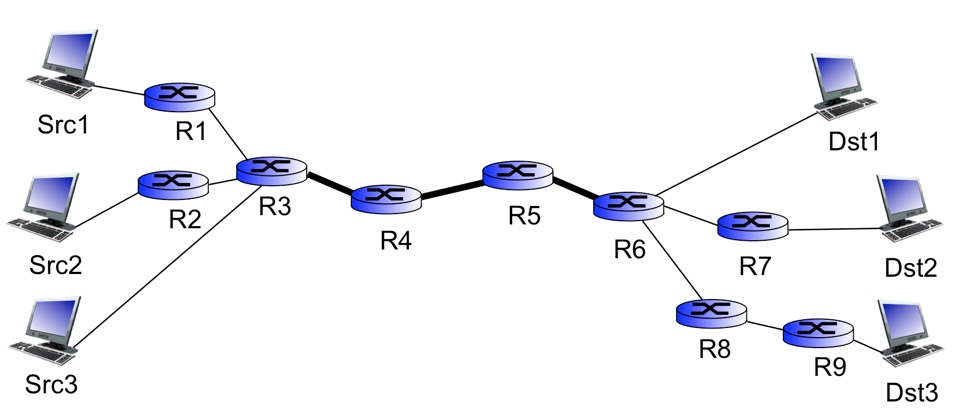
\includegraphics[width=\linewidth]{q2.png}
    
  \end{subfigure}
  \caption{Question 3 Network}
  \label{fig:coffee}
\end{figure}


$\\ \\$$\\ \\$


Propagation delay(the same for all links):

\begin{equation}
    d_{prop} = \frac{link's length }{propagation speed}
\end{equation}
\begin{equation}
    d_{prop} = \frac{300\ m}{2 * 10^8\ m/s}
\end{equation}
\begin{equation}
    d_{prop} = \frac{3 * 10^2\ m}{2 * 10^8\ m/s}
\end{equation}
\begin{equation}
    d_{prop} = \frac{3}{2} * 10^{2-8}\ s
\end{equation}
\begin{equation}
    d_{prop} = 1.5 * 10^{-6}\ s
\end{equation}
\begin{equation}
    \textcolor{red}{d_{prop} = 1.5\ \mu s}
\end{equation}

$\\$
There are six links on the source 1 path and seven links on the source 2 and 3 paths

\begin{equation}
    \textcolor{red}{
    Source1\ delay\ =\ 6 * (d_{prop}) + d_{trans}{\ individual} + d_{trans}{\ shared}}
\end{equation}
\begin{equation}
\textcolor{red}{
    Source2\ delay\ =\ 7 * (d_{prop}) + d_{trans}{\ individual} + d_{trans}{\ shared}}
\end{equation}
\begin{equation}
\textcolor{red}{
    Source3\ delay\ =\ 7 * (d_{prop}) + d_{trans}{\ individual} + d_{trans}{\ shared}}
\end{equation}


Size of the packet of sources 1 and 2 is the same, therefore, they have the same delay value. 

Transmission delay for links 1 and 3 (individual part):

\begin{equation}
    d_{trans}{ind} =\ \frac{L}{R} = \frac{3\ Kb}{0.5\ Gbps} = 6 * 10 ^{3-9}\ s = \textcolor{red}{6\ \mu s}
\end{equation}

Transmission delay for link 2 (individual part):

\begin{equation}
    d_{trans}{ind} =\ \frac{L}{R} = \frac{6\ Kb}{0.5\ Gbps} = 12 * 10 ^{3-9}\ s = \textcolor{red}{12\ \mu s}
\end{equation}

Transmission delay for link 1 and 3 (shared part):
\begin{equation}
    d_{trans}{shared} = \ \frac{L}{R} = \frac{3\ Kb}{\frac{3\ kb}{(3 + 6 + 3) Kb} * 8\ Gbps}
\end{equation}
\begin{equation}
    d_{trans}{shared} = \ \frac{L}{R} = \frac{3\ Kb}{\frac{3\ kb}{12 Kb} * 8\ Gbps}
\end{equation}
\begin{equation}
    d_{trans}{shared} = \ \frac{L}{R} = \frac{3\ Kb}{ \frac{1}{4}* 8\ Gbps}
\end{equation}
\begin{equation}
    d_{trans}{shared} = \ \frac{L}{R} = \frac{3\ Kb}{2\ Gbps}
\end{equation}
\begin{equation}
    d_{trans}{shared} = \ \frac{L}{R} = \frac{3}{2} * 10 ^{3 - 9}\ s
\end{equation}
\begin{equation}
    d_{trans}{shared} = \ \frac{L}{R} = 1.5 * 10 ^{-6}\ s
\end{equation}
\begin{equation}
    \textcolor{red}{d_{trans}{shared} = \ \frac{L}{R} = 1.5\ \mu s}
\end{equation}

Transmission delay for link 2 (shared part):

\begin{equation}
    d_{trans}{shared} = \ \frac{L}{R} = \frac{6\ Kb}{\frac{6\ kb}{(3 + 6 + 3) Kb} * 8\ Gbps}
\end{equation}
\begin{equation}
    d_{trans}{shared} = \ \frac{L}{R} = \frac{6\ Kb}{\frac{6\ kb}{12 Kb} * 8\ Gbps}
\end{equation}
\begin{equation}
    d_{trans}{shared} = \ \frac{L}{R} = \frac{6\ Kb}{ \frac{1}{2}* 8\ Gbps}
\end{equation}
\begin{equation}
    d_{trans}{shared} = \ \frac{L}{R} = \frac{6\ Kb}{4\ Gbps}
\end{equation}
\begin{equation}
    d_{trans}{shared} = \ \frac{L}{R} = \frac{6}{4} * 10 ^{3 - 9}\ s
\end{equation}
\begin{equation}
    d_{trans}{shared} = \ \frac{L}{R} = 1.5 * 10 ^{-6}\ s
\end{equation}
\begin{equation}
    \textcolor{red}{d_{trans}{shared} = \ \frac{L}{R} = 1.5\ \mu s}
\end{equation}



Putting the values into the equations:

\begin{equation}
    
    Source1\ delay\ =\ 6 * (1.5\ \mu s) + (\#  individual\ links = 3)*(6\ \mu s) + (\# shared\ links = 3)*(1.5\ \mu s)
\end{equation}
\begin{equation}
    Source2\ delay\ =\ 7 * (1.5\ \mu s) + (\# individual\ links = 4)*(12\ \mu s) + (\# shared\ links = 3)*(1.5\ \mu s)
\end{equation}
\begin{equation}
    Source3\ delay\ =\ 7 * (1.5\ \mu s) + (\# individual\ links = 4)*(6\ \mu s) + (\# shared\ links = 3)*(1.5\ \mu s)
\end{equation}


Final answer(item a). 
a. Each of the 3 sources of traffic generates a message containing 1 packet.
The end-to-end delay for one packet is:

\begin{equation}
    Source1\ delay\ =\ 6 * (1.5\ \mu s) + (3)*(6\ \mu s) + (3)*(1.5\ \mu s) = \textcolor{red}{31.5\ \mu s}
\end{equation}
\begin{equation}
    Source2\ delay\ =\ 7 * (1.5\ \mu s) + (4)*(12\ \mu s) + (3)*(1.5\ \mu s) = \textcolor{red}{ 63\ \mu s}
\end{equation}
\begin{equation}
    Source3\ delay\ =\ 7 * (1.5\ \mu s) + (4)*(6\ \mu s) + (3)*(1.5\ \mu s) = \textcolor{red}{39\ \mu s}
\end{equation}

$\\$
\hline

$\\ \\$



b. Each of the 3 sources of traffic generates a message containing 200 packets.

The end-to-end delay in this scenario is the end-to-end delay of the first package plus the last link transmission delay of the remaining packages. So, using the data from the item a, we have that:
\begin{equation}
    Source1\ end\ to\ end\ delay\ (1\ pkt)\  = \textcolor{red}{31.5\ \mu s}
\end{equation}
\begin{equation}
    Source2\ end\ to\ end\ delay\ (1\ pkt)\  = \textcolor{red}{ 63\ \mu s}
\end{equation}
\begin{equation}
    Source3\ end\ to\ end\ delay\ (1\ pkt)\  = \textcolor{red}{39\ \mu s}
\end{equation}

If we look on the network image of this question, we will see that the last link of every path is an "individual link", which means the transmission delay for the remaining packages is made of the individual link delay, also calculated on item a.

Transmission delay for links 1 and 3 (individual part):

\begin{equation}
    d_{trans}{ind} =\ \frac{L}{R} = \frac{3\ Kb}{0.5\ Gbps} = 6 * 10 ^{3-9}\ s = \textcolor{red}{6\ \mu s}
\end{equation}

Transmission delay for link 2 (individual part):

\begin{equation}
    d_{trans}{ind} =\ \frac{L}{R} = \frac{6\ Kb}{0.5\ Gbps} = 12 * 10 ^{3-9}\ s = \textcolor{red}{12\ \mu s}
\end{equation}

Therefore the end-to-end delay of each source is:
\begin{equation}
    Source1\ delay\ = (31.5\ \mu s) + (\# pkts -1) * d_{trans}{individual}
\end{equation}
\begin{equation}
    Source2\ delay\ = (63\ \mu s)  + (\# pkts -1) * d_{trans}{individual}
\end{equation}
\begin{equation}
    Source3\ delay\ = (39\ \mu s)  + (\# pkts -1) * d_{trans}{individual}
\end{equation}

\begin{equation}
    Source1\ delay\ = (31.5\ \mu s) + (200 -1) * (6\ \mu s) = \textcolor{red}{ 1,225.3\ \mu s} = \textcolor{red}{1.2553\ ms}
\end{equation}
\begin{equation}
    Source2\ delay\ = (63\ \mu s)  + (200 -1) * (12\ \mu s) = \textcolor{red}{2,451\ \mu s} = \textcolor{red}{2.451\ ms}
\end{equation}
\begin{equation}
    Source3\ delay\ = (39\ \mu s)  + (200 -1) * (6\ \mu s) = \textcolor{red}{1,233\ \mu s} = \textcolor{red}{1.233\ ms}
\end{equation}

$\\$

\hline
$\\$


Notes: 
1.	Refer to lecture2, slides 9 and 15, end-to-end delay for a message containing several packets. 
2.	When a node transmits a packet, it doesn’t need to wait for the last packet to be propagated along the link. As soon as one packet is transmitted into the link, the node can start transmitting the next packet.

$\\$
$\\$



\end{document}

